\documentclass[12pt, a4paper,twocolumn]{article}%klasa article papier a4 czcionka 12, dwie kolumny
\usepackage[final]{graphicx} %wstawianie obrazków
\usepackage{tabularx} %tabela
\usepackage{polski} %znaki polskie
\usepackage[compact]{titlesec} %do odległości między sekcjami
%Odległości między sekcjami
\titlespacing{\section}{0pt}{1ex}{1ex}
\titlespacing{\subsection}{0pt}{0.5ex}{0ex}
\titlespacing{\subsubsection}{0pt}{0.5ex}{0ex}
%Strona tytułowa - dane
\title{Chmury punktów - Wprowadzenie}
\author{Konrad Bedełek}
\date{19.05.2022}


\begin{document}

	%Strona tytułowa
	\begin{titlepage}
	\maketitle
	\thispagestyle{empty}
	\end{titlepage}

	%Abstract
	\begin{abstract}
	W ostatnich latach popularnym stały się zagadnienia związane ze skanowaniem 3D. Jednym z najpopularniejszych metod przedstawienia wyników skanowania 3D jest chmura punktów. W niniejszym artykule przedstawiono czym jest chmura punktów oraz w jakich celach znajduje ona zastosowanie.
	\end{abstract}

	\section{Wprowadzenie}
	Na podstawie skaningu laserowego, bądź pomiarów fotogrametrycznych, które są aktualnie jednymi z najszybszych i najskuteczniejszych technik pomiarowych, tworzymy gotowy produkt jakim jest chmura punktów.\cite{kowal1}

	\subsection{Czym jest chmura punktów}
	Chmura punktów to zbiór punktów stanowiący geometryczną reprezentację skanowanego obiektu. Chmury punktów zazwyczaj są tak gęste, że wydaje się one tworzyć powierzchnię ciągłą. Dopiero po znacznym powiększeniu okazuje się że jest to zbiór pojedynczych punktów. Punkty chmury punktów nie są jednak interpretowane jako niepowiązane ze sobą obiekty, a jako spójna struktura. Wiele programów dzięki umiejętności wyznaczenia normalnej daje możliwość wyszukiwania w chmurze płaszczyzn, cylindrów, kul, a nawet bardzo złożonych obiektów bryłowych. Stosując aparat wbudowany w skaner bądź zewnętrzny, można nadać chmurze punktów wartości RGB pikseli z matrycy aparatu. Dzięki temu chmura zyskuje realistyczny charakter i doskonale nadaje się do wizualizacji.\linebreak Poniżej przedstawiono przykładową chmurę punktów z nałożonymi kolorami.

	%Wstaw obrazek
	\begin{figure}[h!]%Wstaw go w tym miejscu właśnie
	\begin{center}%Wycentruj
	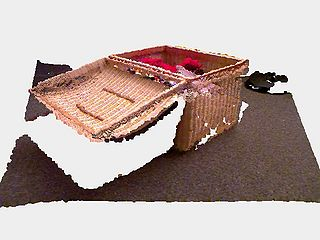
\includegraphics[width=0.4\textwidth]{point_cloud.jpg} %Ciut za duże więc zmniejszyć trzeba
	\caption{Przykładowa chmura punktów}

	\end{center}
	\end{figure}



	\subsection{Zastosowania chmury punktów}
	Chmury punktów znajdują szerokie zastosowanie m.in. w przemyśle, sztuce i robotyce. Poniżej przedstawiono kilka popularnych zastosowań oraz formatów zapisu chmur punktów.			\cite{kowal2}\cite{hans1}

	% lista
	\begin{itemize}
	\setlength\itemsep{0em} % odległości między itemami
	\item Dokumentowanie zabytków
	\item Detekcja kolizji
	\item Inwentaryzacje powykonawcze oraz pomiary w trakcie procesu budowlanego
	\item Badanie objętości mas ziemnych
	\item Dokumentacja techniczna części maszyn
	\end{itemize}
	%wstaw tabelę
	\begin{table}[h!]%wstaw tabelę w miejscu jak w kodzie
	\begin{tabularx}{0.6\textwidth} { |X|X| }
	\hline
	Skrót  & Format\\
	\hline
	.POD & Pointools and Bentley\\
	\hline
	.PCG & AutoDesk\\
	\hline
	.FLS & Faro\\
	\hline
	.PTS, XYZ & standard ASCII\\
	\hline

	\end{tabularx}
	\caption{Formaty chmur punktów}
	\end{table}
	
	\pagebreak %przejdź do następnej strony
	\onecolumn %now one column
	\listoftables %lista tabel
	\listoffigures %lista obrazków

	%bibliografia
	\begin{thebibliography}{9}
	\bibitem{kowal1} Kowalski A. Technologia skanowania 3D, Warszawa, 2018
	\bibitem{kowal2} Kowalski J. Techniki zapisu danych, Warszawa, 2015
	\bibitem{hans1} Copernicus H. O obrotach dział Niemieckich, Berlin, 1914
	\end{thebibliography}

\end{document}